% The layers an analysis depends on, and the four ways to talk to a system.
% ---------------------------------------------------------------------------
% style.tex --- shared preamble for every figure in book/figures/tikz/
%
% One style for all figures: Latin Modern, thin black lines, a light grey
% fill, and one accent colour used only to mark what is untrusted or wrong.
% Build with scripts/build_figures.sh; see book/figures/README.md.
% ---------------------------------------------------------------------------
\documentclass[tikz,border=6pt]{standalone}
\usepackage[T1]{fontenc}
\usepackage{lmodern}
\usetikzlibrary{arrows.meta,positioning,shapes.geometric,calc,fit,backgrounds}

\hyphenpenalty=10000   % short lines in boxes: ragged, never hyphenated

\definecolor{lightgrey}{gray}{0.92}
\definecolor{accent}{HTML}{9B2D20}

\tikzset{
  every picture/.style={
    line width=0.6pt,
    font=\small,
    >={Stealth[length=5pt,width=4pt]},
    node distance=14pt and 24pt,
  },
  % shapes
  box/.style={draw, rectangle, inner xsep=8pt, inner ysep=5pt,
              minimum height=22pt, align=center},
  grey/.style={box, fill=lightgrey},
  rounded/.style={box, rounded corners=9pt},
  decision/.style={draw, diamond, aspect=2.4, inner sep=1.5pt, align=center},
  group/.style={draw, dashed, rounded corners=5pt, inner sep=7pt},
  % text
  tag/.style={font=\footnotesize, align=center, inner sep=2pt},
  note/.style={font=\footnotesize\itshape, align=center, inner sep=2pt},
  code/.style={font=\small\ttfamily},
  codetag/.style={font=\footnotesize\ttfamily, align=center, inner sep=2pt},
  title/.style={font=\small\scshape, align=center, inner sep=2pt},
  % lines
  arrow/.style={->},
  back/.style={->, dashed},
  thin/.style={line width=0.4pt, gray},
  % the one accent, for what is untrusted, wrong or missing
  bad/.style={accent},
  badbox/.style={box, draw=accent, text=accent},
}

\begin{document}
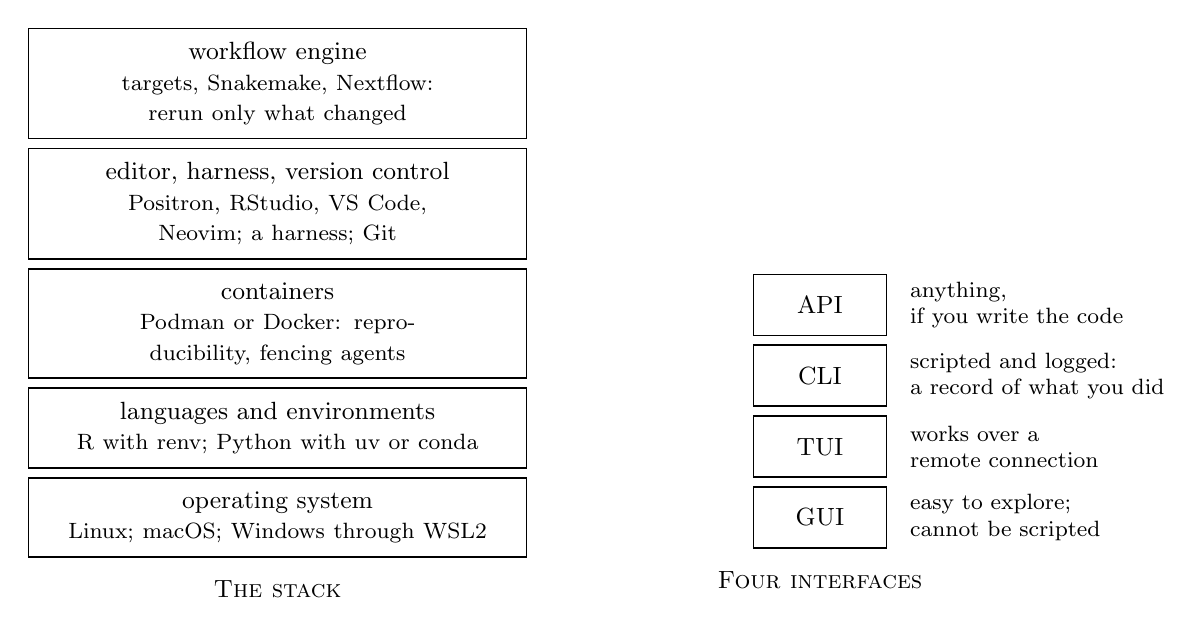
\begin{tikzpicture}[node distance=3pt,
                    layer/.style={box, text width=164pt, align=center, minimum height=26pt}]
  \node[layer] (os) at (0,0) {operating system\\ \footnotesize Linux; macOS; Windows through WSL2};
  \node[layer, above=of os] (lang) {languages and environments\\ \footnotesize R with renv; Python with uv or conda};
  \node[layer, above=of lang] (cont) {containers\\ \footnotesize Podman or Docker: reproducibility, fencing agents};
  \node[layer, above=of cont] (ed) {editor, harness, version control\\ \footnotesize Positron, RStudio, VS Code, Neovim; a harness; Git};
  \node[layer, above=of ed] (wf) {workflow engine\\ \footnotesize targets, Snakemake, Nextflow: rerun only what changed};
  \node[title, below=6pt of os] {The stack};
  % interfaces
  \node[box, minimum width=48pt] (gui) at (196pt,0) {GUI};
  \node[box, minimum width=48pt, above=of gui] (tui) {TUI};
  \node[box, minimum width=48pt, above=of tui] (cli) {CLI};
  \node[box, minimum width=48pt, above=of cli] (api) {API};
  \node[tag, right=6pt of gui, anchor=west, align=left] {easy to explore;\\cannot be scripted};
  \node[tag, right=6pt of tui, anchor=west, align=left] {works over a\\remote connection};
  \node[tag, right=6pt of cli, anchor=west, align=left] {scripted and logged:\\a record of what you did};
  \node[tag, right=6pt of api, anchor=west, align=left] {anything,\\if you write the code};
  \node[title, below=6pt of gui] {Four interfaces};
\end{tikzpicture}
\end{document}
